\documentclass[compress,10pt]{beamer}
\useoutertheme[footline=authorinstitutetitle]{miniframes}
\usecolortheme{whale}
\usecolortheme{orchid}
\useinnertheme{rounded}

\setbeamerfont{block title}{size={}}

%\documentclass[compress]{beamer}
%\usepackage{beamerthemeproyxetex}


%\useoutertheme[footline=authorinstitutetitle]{miniframes}
%\usecolortheme{whale}
%\usecolortheme{orchid}
%\useinnertheme{rounded}

\usepackage{placeins}

\title{FoLiA: Format for Linguistic Annotation}
\author{Maarten van Gompel \\ Radboud University Nijmegen}
\date{20-01-2012}
\usepackage{graphicx}
\usepackage{listings}
\usepackage{color}
\lstset{% general command to set parameter(s)
basicstyle=\footnotesize,
keywordstyle=\color{black}\bfseries\underbar,
identifierstyle=\color{black}\bfseries\underbar,
stringstyle=\ttfamily,
}

\def\raccoon{
\makebox[\linewidth][c]{\includegraphics[width=70pt]{/home/proycon/Pictures/All/raccoon.pdf}\FloatBarrier}
}
\def\smallraccoon{
\makebox[\linewidth][c]{\includegraphics[width=30pt]{/home/proycon/Pictures/All/raccoon.pdf}\FloatBarrier}
}


\begin{document}

\begin{frame}
	\titlepage\smallraccoon
\end{frame}

\section{Introduction}
\subsection{Introduction}

\begin{frame}{Introduction}

	\begin{block}{What is FoLiA?}
		\begin{itemize}
			\item Generalised XML-based format for a wide variety of linguistic annotation
		\end{itemize}				
	\end{block}	

	\begin{block}{Characteristics}
		\begin{itemize}
			\item \textbf{Generalised} paradigm -- Single universal paradigm applicable to all kinds of annotations; as few ad-hoc provisions as possible. Not commited to any label set.
			\item \textbf{Extensible} -- Unsupported annotation types can be added fairly easily.
			\item \textbf{Expressive} -- Verbose expression of annotations, their annotators, timestamps, etc... Moreover, support for \emph{alternative} annotations. 
			\item \textbf{Formalised} -- Validation on two levels: shallow and deep. The latter validates the used label set and allows for links with for instance ISOcat.			
		\end{itemize}				
	\end{block}

\end{frame}

\section{Features}
\subsection{Features}

\begin{frame}

	\begin{block}{Intended Applications}
		\begin{itemize}
			\item as a corpus storage format
			\item as a language resource exchange format 
		\end{itemize}				
	\end{block}

	\begin{block}{Properties}
		\begin{itemize}	
			\item One document, one text, one XML file -- containing all annotations.
			\item Annotation types and label sets must be declared in the document header
			\item Document metadata can be either included in the file (limited), or by reference to external CMDI or IMDI (preferred)
		\end{itemize}
	\end{block}
	
	
\end{frame}	
	
\subsection{Motivation \& Dissemination}	
	
\begin{frame}
	\begin{block}{Why (yet) another format?}
		\begin{itemize}
			\item Many ad-hoc and legacy annotation formats (CGN, Tadpole column format)
			\item Many theoretic and specialised annotation formats with limited scope (LAF, SynAF, MAF, TEI)
			\item Bottom-up rather than top-down development: FoLiA arose from practical need, immediately developed alongside practical programming libraries and applications. 
			\item De-facto-standard: D-COI XML
		\end{itemize}
	\end{block}
	
	\begin{block}{Dissemination}
		\begin{itemize}	
			\item SoNaR
			\item TTNWW
			\item DutchSemCor
			\item Valkuil.net
			\item Frog \& Ucto
		\end{itemize}			
	\end{block}

\end{frame}
   
       
\section{Paradigm}

\subsection{Annotation Categories}

\begin{frame}{Paradigm}
    \begin{block}{Paradigm: Annotation Categories}
        Four categories of annotation:    
        \begin{itemize}            
            \item \textbf{Structure Annotation} - Elements denoting document structure
            \begin{itemize}
                \item {\footnotesize E.g: Divisions, Header, Paragraphs, Sentences, Lists, Figures, Gaps, Quote }
            \end{itemize}
            \item \textbf{Token Annotation} - Linguistic Annotations pertaining to a single token (inline annotation)
            \begin{itemize}
                \item {\footnotesize E.g: Part of Speech Annotation, Lemma Annotation, Lexical Semantic Sense Annotation }
            \end{itemize}
            \item \textbf{Span Annotation} - Linguistic Annotations spanning over multiple tokens (standoff annotation)
            \begin{itemize}
                \item {\footnotesize E.g: Syntactic Parses, Dependency Relations, Entities/Multi-word Units}
            \end{itemize}
			\item \textbf{Subtoken Annotation} - Linguistic Annotations pertaining to a subpart of a token (standoff annotation)
            \begin{itemize}
                \item {\footnotesize E.g: Morphology}
            \end{itemize}
        \end{itemize}           
    \end{block}
\end{frame}

\subsection{Attributes}

\begin{frame}
        %\frametitle{Paradigm: Schematic}
        \begin{center}
        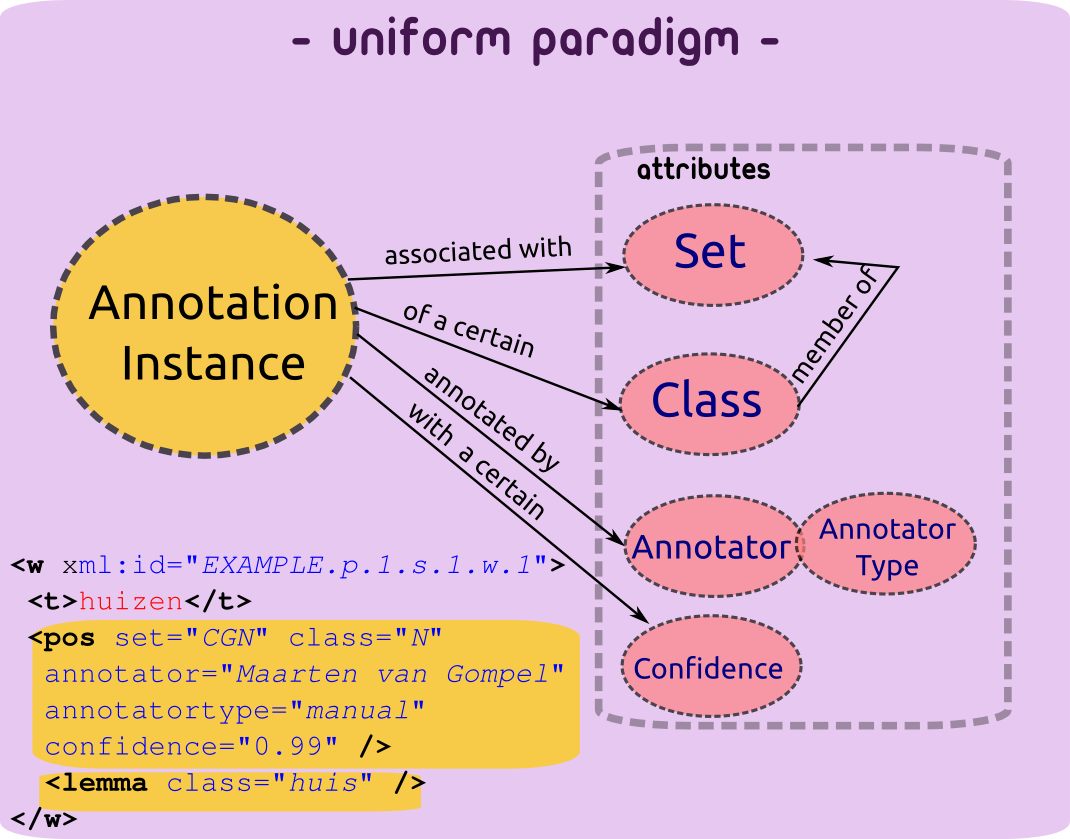
\includegraphics[width=90.0mm]{paradigm.png}
        \end{center}
\end{frame}


\section{Format}

\subsection{Document skeleton}

\begin{frame}[fragile]
\frametitle{Format}
\begin{lstlisting}[language=xml]
<?xml version="1.0" encoding="utf-8"?>
<FoLiA xmlns="http://ilk.uvt.nl/FoLiA"
  xmlns:xsi="http://www.w3.org/2001/XMLSchema-instance"
  xml:id="example">
  <metadata type="cmdi" src="example.cmdi">    
    <annotations>
      ...
    </annotations>   
  </metadata>
  <text xml:id="example.text">
     ...
  </text>
</FoLiA>  
\end{lstlisting}
\end{frame}

\subsection{Structure Annotation}

\begin{frame}[fragile]
	\begin{example}
\begin{lstlisting}[language=xml]
<p xml:id="TEST.p.1">
	<t>This is a test. It has two sentences.</t>
	<s xml:id="TEST.p.1.s.1">        
	    <t>This is a test.</t>
	    <w xml:id="TEST.p.1.s.1.w.1"><t>This</t></w>
	    <w xml:id="TEST.p.1.s.1.w.2"><t>is</t></w>
	    ..
	</s><s xml:id="TEST.p.1.s.2">...</s>                
</p>                
\end{lstlisting}    
	\end{example}

    \begin{block}{Characteristics of basic structure}
      \begin{enumerate}
        \item \textbf{Structure Elements}: Paragraphs, Sentences, Words/Tokens  
        \item More: Division, Head, List, ListItem, Figure, Gap...
        \item Unique identifiers
        \item Text content element (t) holds actual text.
      \end{enumerate}
    \end{block}
\end{frame}


%\subsection{Token Annotation}

\begin{frame}[fragile]
    \begin{block}{Token Annotation}
        Token annotation occurs within the scope of a word/token (\emph{w}) element.
    \end{block}
    \begin{example}
       PoS and Lemma Annotation:
\begin{lstlisting}[language=xml]
<w xml:id="example.p.1.s.1.w.2">
    <t>boot</t>
    <pos set="cgn" class="n" 
     annotator="Maarten van Gompel" annotatortype="manual" />
    <lemma set="english-lemmas" class="boot" />
    <sense set="cornetto" class="D_N12345" annotator="supwsd1" 
     annotatortype="auto" confidence="0.65" />
</w>                         
\end{lstlisting}        
    \end{example}
\end{frame}

\begin{frame}[fragile]

	\begin{block}{Token Annotations with subsets}
		For all annotation types; \textbf{subsets} can be used for more refined annotations.  
	\end{block}
	
	\begin{example}
\begin{lstlisting}[language=xml]
<w xml:id="example.p.1.s.1.w.2">
    <t>boot</t>
    <pos set="cgn" class="N(soort,ev,basis,zijn,stan)">
        <feat subset="head" class="N" />
        <feat subset="ntype" class="soort" />
        <feat subset="number" class="ev" />
        <feat subset="degree" class="basis" />
        <feat subset="gender" class="zijd" />
        <feat subset="case" class="stan" />
    </pos>
</w>
\end{lstlisting}   
	\end{example} 

\end{frame}



\subsection{Span Annotation}
        
\begin{frame}
    \begin{block}{Span Annotation}
        \begin{itemize}
            \item Token Annotation is not sufficient, some annotations span over multiple tokens (not necessarily consecutive)
            \item Spanning multiple tokens can produce nesting problems (e.g $A (B C) D$ and $A B (C D)$)                
            \item \textbf{Solution:} Span Annotation using standoff notation
        \end{itemize}        
    \end{block}
    
    \begin{block}{Properties}
    	\begin{itemize}
    	 \item \textbf{Applications:} Syntactic Parses, Chunking, Dependency Relations, Entities/Multi-Word Units    	
         \item \textbf{Layers:} Each type of span annotation is placed within an \emph{annotation layer}, annotation layers are usually embedded within \emph{sentences} (\texttt{s))}
         \item Same paradigm: Set, class, annotator, confidence, etc...
        \end{itemize}
    \end{block}
\end{frame}

\begin{frame}[fragile]
\begin{lstlisting}[language=xml]
<s xml:id="example.p.1.s.1">
  <t>The Dalai Lama greeted him.</t>
  <w xml:id="example.p.1.s.1.w.1"><t>The</t></w>
  <w xml:id="example.p.1.s.1.w.2"><t>Dalai</t></w>
  <w xml:id="example.p.1.s.1.w.3"><t>Lama</t></w>
  <w xml:id="example.p.1.s.1.w.4"><t>greeted</t></w>
  <w xml:id="example.p.1.s.1.w.5"><t>him</t></w>
  <w xml:id="example.p.1.s.1.w.6"><t>.</t></w>
  <entities>
    <entity xml:id="example.p.1.s.1.entity.1" class="person">
        <wref xml:id="example.p.1.s.1.w.2" />
        <wref xml:id="example.p.1.s.1.w.3" />
    </entity>
  </entities>
</s>
\end{lstlisting}                    
\end{frame}

\begin{frame}[fragile]
\begin{lstlisting}[language=xml]
<syntax>
<su xml:id="example.p.1.s.1.su.1" class="s">     
  <su xml:id="example.p.1.s.1.su.1_1" class="np">
      <su xml:id="example.p.1.s.1.su.1_1_1" class="det">
         <wref xml:id="example.p.1.s.1.w.1" />       
      </su>
      <su xml:id="example.p.1.s.1.su.1_1_2" class="pn">
         <wref xml:id="example.p.1.s.1.w.2" />
         <wref xml:id="example.p.1.s.1.w.3" />        
      </su>         
   </su>
 </su>
 <su xml:id="example.p.1.s.1.su.1_2" class="vp"> 
    <su xml:id="example.p.1.s.1.su.1_1_1" class="v">
        <wref xml:id="example.p.1.s.1.w.4" />       
    </su>
    <su xml:id="example.p.1.s.1.su.1_1_2" class="pron">
      <wref xml:id="example.p.1.s.1.w.5" />       
    </su>
 </su>    
</su>
</syntax>
\end{lstlisting}                    
\end{frame}



\section{Tools}

\begin{frame}
	\begin{block}{Tools for working with FoLiA}
		\begin{itemize}
			\item Standard \textbf{XML} facilities: XSLT, XPath
			\item \textbf{Python} library: pynlpl.formats.folia
			\item \textbf{C++} library: libfolia \emph{(Ko van der Sloot)}
		\end{itemize}
	\end{block}
	
	\begin{block}{Applications}
		\begin{itemize}
			\item \textbf{Frog} -- tagger/lemmatisaion/parser suite: FoLiA output (input in later stage).
			\item \textbf{ucto} -- tokeniser: FoLiA input and output.
		\end{itemize}
	\end{block}
	
	\begin{block}{Converters}
		\begin{itemize}
			\item DCOI $\longleftrightarrow$ FoLiA
			\item FoLiA $\longrightarrow$ CSV   (limited)
		\end{itemize}
	\end{block}
\end{frame}


\section{Conclusion}

\begin{frame}
    \begin{block}{Conclusion}
        \begin{itemize}
            \item \textbf{Uniformity:} generic framework with simple paradigm, XML based
            \item \textbf{Expressiveness:} Ability to encode many kinds of linguistic annotation, including structural annotation, alternatives, and corrections
            \item \textbf{Extensibility:} easy to add new annotations with the same paradigm
            \item A variety of tools and converters already available!
        \end{itemize}
    \end{block}
    
    \begin{block}{URLs}
    	\begin{itemize}
    		\item http://ilk.uvt.nl/folia
	    	\item http://github.com/proycon/folia
	    \end{itemize}
    \end{block}

\end{frame}

\section{The End}

\begin{frame}

\raccoon

\begin{center}
\Large{Questions?}
\end{center}

\end{frame}



\section{Extra}

\subsection{Trade-off}


\begin{frame}
	\begin{block}{Trade-off: Expressivity versus Computing Efficiency}		
		\begin{itemize}
    			\item FoLiA aims at expressivity rather than computing efficiency. 
			\begin{itemize}
				\item XML and FoLiA overhead: Not ideal for real-time or resource-constrained applications
				\item \textbf{Conversion} to less expressive, more efficient, formats.
			\end{itemize}			 
		\end{itemize}	
	\end{block}
\end{frame}

\subsection{Annotations}   
   
\begin{frame}
    \begin{block}{Supported Annotations (1/2)}
        FoLiA supports the following linguistic annotations:
        \begin{itemize}
            \item Part-of-Speech tags (with features)
            \item Lemmatisation
            \item Domain tagging
            \item Lexical semantic sense annotation (used in DutchSemCor)
            \item Named Entities / Multi-word units (used in SoNaR)
            \item Syntactic Parses
            \item Dependency Relations            
        \end{itemize}        
    \end{block}
\end{frame}
            
\begin{frame}
    \begin{block}{Supported Annotations (2/2)}
        FoLiA supports the following linguistic annotations:
        \begin{itemize}                       
            \item Chunking
            \item Corrections (used in valkuil.net)
            \item Morphology
            \item Event/Time annotation
            \item Phonetic annotation
        \end{itemize}   
    \end{block}
\end{frame}

        
\subsection{Declarations}

\begin{frame}[fragile]
    \begin{block}{Token Annotation}
        All annotations need to be declared in the metadata:
        \begin{itemize}
            \item Default sets and annotator \emph{may} be predefined at this level
        \end{itemize}
    \end{block}
    \begin{example}
\begin{lstlisting}[language=xml]
<metadata>
 <annotations>
  <token-annotation />
  <pos-annotation set="brown" annotator="Maarten van Gompel"
    annotatortype="manual"/>
  <lemma-annotation />
 </annotations>
</metadata>                     
\end{lstlisting}        
    \end{example}
\end{frame}

\subsection{Alternatives}

\begin{frame}[fragile]
\frametitle{Alternative Token Annotations}

Annotations of the same type, but different sets need \emph{not} be alternatives.

\begin{lstlisting}[language=xml]
<w xml:id="example.p.1.s.1.w.2">
    <t>luid</t>
    <pos set="brown" class="jj" />
    <pos set="cgn" class="adj" />
</w>                         
\end{lstlisting}        

There can be only one of the same set though, this is illegal and requires usage of alternatives instead:

\begin{lstlisting}[language=xml]
<w xml:id="example.p.1.s.1.w.2">
    <t>luid</t>
    <pos set="cgn" class="adj" />
    <pos set="cgn" class="adv" />
</w>                         
\end{lstlisting}   

\end{frame}


\begin{frame}[fragile]
\frametitle{Alternative Token Annotations}

Encodes mutually exclusive alternative annotations. Any annotations that are not alternatives are considered ``selected''.

\begin{lstlisting}[language=xml]
<w xml:id="example.p.1.s.1.w.2">
    <t>bank</t>
    <sense set="wordnet3.0" class="bank%1:17:01:"    
     annotator="Maarten van Gompel" annotatortype="manual" 
     confidence="0.8">
     sloping ground near water</sense>
    <alt xml:id="example.p.1.s.1.w.2.alt.1">
     <sense set="wordnet3.0" class="bank%1:14:01:"
      annotator="WSDsystem" annotatortype="auto" 
      confidence="0.6">     
      financial institution</sense> 
    </alt>
</w>                         
\end{lstlisting}        

\end{frame}

\begin{frame}[fragile]
\frametitle{Alternative Token Annotations}

All token annotations grouped as one alternative are considered dependent. Multiple alternatives are always independent:

\begin{lstlisting}[language=xml]
<w xml:id="example.p.1.s.1.w.2">
    <t>vlieg</t>
    <pos class="N" />
    <lemma class="vlieg" />
    <alt xml:id="example.p.1.s.1.w.2.alt.1">
        <pos class="V" />
        <lemma class="vliegen" />
    </alt>
</w>                         
\end{lstlisting}        

\end{frame}






\end{document}
